\documentclass[t,aspectratio=169,xcolor=dvipsnames]{beamer}
\usetheme{SimplePlusAIC}

\usepackage{graphicx}
\usepackage{booktabs}
\usepackage{svg}
\usepackage{tcolorbox}
\usepackage{tikz}
\usetikzlibrary{shapes.geometric, arrows, positioning, fit, calc}
\usepackage{makecell}
\usepackage{listings}

\newcommand*{\defeq}{\stackrel{\text{def}}{=}}
\usepackage{setspace}
\usepackage[T1]{fontenc}
\usepackage{helvet}
\usepackage{amsmath}
\usepackage{ragged2e}
\usepackage{gensymb}

\usepackage[svgnames,table]{xcolor}
\arrayrulecolor{black}
\setlength{\arrayrulewidth}{0.20mm}
\renewcommand{\arraystretch}{1.35}

% Highlight istilah penting: bold + merah
\newcommand{\tem}[1]{\textbf{\textcolor{red}{#1}}}

% Konfigurasi listings (jika ada kode)
\lstset{
    basicstyle=\ttfamily\small,
    breaklines=true,
    columns=fullflexible,
    frame=none
}

\title[Pengayaan OS]{Pengayaan: Keamanan, Hak Akses, RAID \& Docker}
\subtitle{Week 13: Hak Akses File, Virus dan Security, RAID, serta Container}
\author[informatika-itera.github.io/os]{informatika-itera.github.io/os}
\institute[ITERA]{Program Studi Teknik Informatika \\ Institut Teknologi Sumatera}
\date{\textcolor{nyublue}{2026}}

\AtBeginSection[]{
    \begin{frame}[plain]
        \vfill
        \centering
        {\usebeamerfont{title}\color{nyublue}\Huge \insertsectionhead\par}
        \vfill
    \end{frame}
}

\begin{document}

% 1. Title frame
\begin{frame}
    \titlepage
\end{frame}

% 2. Outline frame
\begin{frame}
    \frametitle{Outline}
    \tableofcontents
\end{frame}

% 3. Capaian Pembelajaran
\begin{frame}[shrink=5]
    \frametitle{Capaian Pembelajaran}
    \framesubtitle{Tujuan setelah pertemuan selesai}
    \small
    \begin{enumerate}
        \item Memahami model hak akses file di Linux (rwx, owner/group/others).
        \item Mengenal berbagai jenis malware dan bagaimana OS melindungi diri.
        \item Memahami konsep RAID dan perbedaan level-levelnya.
        \item Menjelaskan perbedaan container dan VM serta konsep dasar Docker.
    \end{enumerate}
    \vspace{0.5cm}
    \begin{exampleblock}{Fokus Kelas Ini}
        Kita fokus pada empat topik pengayaan: \tem{Hak Akses}, \tem{Keamanan OS}, \tem{RAID}, dan \tem{Docker}.
    \end{exampleblock}
\end{frame}

%================================================
% BAGIAN 1: HAK AKSES
%================================================
\section{Hak Akses di Linux}

%--- Slide 1: Motivasi ---
\begin{frame}
    \frametitle{Mengapa Hak Akses Penting?}
    \framesubtitle{Dari Week 12 kita tahu file disimpan -- tapi siapa yang boleh mengaksesnya?}

    \begin{columns}[T]
        \column{0.48\textwidth}
        \begin{block}{Masalah}
            \small
            \begin{itemize}
                \item Dalam sistem multi-user, banyak orang bisa pakai komputer yang sama.
                \item File A milik Budi -- jangan sampai Siti bisa baca atau ubah.
                \item OS harus bisa menjawab: \tem{who can do what to which file?}
            \end{itemize}
        \end{block}

        \column{0.48\textwidth}
        \begin{exampleblock}{Analogi: Kantor Sewaan}
            \small
            \begin{itemize}
                \item Setiap karyawan punya ruangan sendiri (home directory).
                \item Beberapa ruangan bersifat umum (shared folder).
                \item Ada dokumen rahasia yang hanya boleh dibaca direktur.
                \item Resepsionis cek kartu akses setiap kali masuk ruangan.
            \end{itemize}
        \end{exampleblock}
    \end{columns}
\end{frame}

%--- Slide 2: Model Unix Permissions ---
\begin{frame}[shrink=5]
    \frametitle{Model Unix: Owner, Group, Others}
    \framesubtitle{Tiga kategori pengguna + tiga jenis izin}

    \begin{columns}[T]
        \column{0.55\textwidth}
        \begin{block}{Tiga Kategori}
            \small
            \begin{itemize}
                \item \textbf{Owner (u)} -- Pemilik file (biasanya pembuat).
                \item \textbf{Group (g)} -- Semua anggota grup yang sama.
                \item \textbf{Others (o)} -- Semua pengguna lain di sistem.
            \end{itemize}
        \end{block}

        \vspace{0.15cm}
        \begin{block}{Tiga Jenis Izin}
            \small
            \begin{itemize}
                \item \textbf{r (read)} -- Baca isi file / lihat daftar direktori.
                \item \textbf{w (write)} -- Ubah file / buat-hapus file di direktori.
                \item \textbf{x (execute)} -- Jalankan file sebagai program / masuk ke direktori.
            \end{itemize}
        \end{block}

        \column{0.40\textwidth}
        \begin{exampleblock}{Contoh: \texttt{ls -l}}
            \small
            \texttt{-rwxr-xr--} \\
            \vspace{0.1cm}
            \begin{tabular}{ll}
                Owner: & rwx (baca-tulis-jalan) \\
                Group: & r-x (baca-jalan) \\
                Other: & r-- (baca saja) \\
            \end{tabular}
            \vspace{0.2cm}
            \begin{itemize}
                \item[$\to$] Owner bisa edit dan jalankan.
                \item[$\to$] Orang lain cuma bisa baca.
            \end{itemize}
        \end{exampleblock}
    \end{columns}
\end{frame}

%--- Slide 3: Numeric Notation ---
\begin{frame}[shrink=5]
    \frametitle{Numeric Notation (Mode Oktal)}
    \framesubtitle{Cara cepat menulis permission dengan angka}

    \begin{columns}[T]
        \column{0.48\textwidth}
        \begin{center}
            \begin{tabular}{ccl}
                \toprule
                \textbf{Angka} & \textbf{Biner} & \textbf{Izin} \\
                \midrule
                7 & 111 & rwx \\
                6 & 110 & rw- \\
                5 & 101 & r-x \\
                4 & 100 & r-- \\
                0 & 000 & --- \\
                \bottomrule
            \end{tabular}
        \end{center}

        \column{0.48\textwidth}
        \begin{block}{Rumus}
            \small
            \texttt{chmod 754 file} = \\
            Owner: 7 (rwx) \\
            Group: 5 (r-x) \\
            Other: 4 (r--)
        \end{block}

        \vspace{0.2cm}
        \begin{exampleblock}{Contoh Umum}
            \small
            \begin{itemize}
                \item \texttt{755} -- script/program (rwxr-xr-x)
                \item \texttt{644} -- dokumen biasa (rw-r--r--)
                \item \texttt{600} -- file pribadi (rw-------)
                \item \texttt{700} -- direktori pribadi (rwx------)
            \end{itemize}
        \end{exampleblock}
    \end{columns}
\end{frame}

%--- Slide 4: Symbolic Notation ---
\begin{frame}[shrink=5]
    \frametitle{Symbolic Notation: chmod [who] [+/-/=] [perms]}
    \framesubtitle{Mengubah permission dengan simbol, bukan angka}

    \begin{columns}[T]
        \column{0.52\textwidth}
        \begin{block}{Format Umum}
            \small
            \texttt{chmod [who][+/-/=][permissions] file}
            \vspace{0.1cm}
            \begin{itemize}
                \item \textbf{Who}: \texttt{u} (user), \texttt{g} (group), \texttt{o} (other), \texttt{a} (all).
                \item \textbf{Operator}: \texttt{+} tambah, \texttt{-} hapus, \texttt{=} set persis.
                \item \textbf{Perms}: \texttt{r}, \texttt{w}, \texttt{x}.
            \end{itemize}
        \end{block}

        \vspace{0.15cm}
        \begin{block}{Kombinasi}
            \footnotesize
            \begin{itemize}
                \item \texttt{chmod u+x file} -- tambah execute untuk user.
                \item \texttt{chmod go-rw file} -- hapus read+write untuk group \& other.
                \item \texttt{chmod a=r file} -- semua cuma bisa baca.
            \end{itemize}
        \end{block}

        \column{0.44\textwidth}
        \begin{exampleblock}{Contoh Langkah demi Langkah}
            \footnotesize
            Awal: \texttt{-rwxr-xr--} (mode 754)
            \vspace{0.1cm}
            \begin{enumerate}
                \item \texttt{chmod u-w} \\[-2pt]
                \texttt{-r-xr-xr--} $\leftarrow$ user kehilangan write
                \vspace{0.08cm}
                \item \texttt{chmod 755} \\[-2pt]
                \texttt{-rwxr-xr-x} $\leftarrow$ other dapat execute
                \vspace{0.08cm}
                \item \texttt{chmod 644} \\[-2pt]
                \texttt{-rw-r--r--} $\leftarrow$ user \& group kehilangan execute
            \end{enumerate}
        \end{exampleblock}
    \end{columns}
\end{frame}

%--- Slide 4: Special Bits ---
\begin{frame}
    \frametitle{Special Bits: Setuid, Setgid, Sticky Bit}
    \framesubtitle{Istimewa -- izin di luar rwx biasa}

    \begin{columns}[T]
        \column{0.48\textwidth}
        \begin{block}{SUID (Set User ID) -- \texttt{chmod u+s}}
            \small
            \begin{itemize}
                \item Program jalan dengan \textbf{privilege pemiliknya}, bukan yang menjalankan.
                \item Contoh: \texttt{passwd} -- perlu akses root untuk ubah password, tapi user biasa bisa jalankan.
                \item Tampil sebagai \texttt{s} di posisi x owner: \texttt{-rwsr-xr-x}.
            \end{itemize}
        \end{block}

        \column{0.48\textwidth}
        \begin{block}{SGID \& Sticky Bit}
            \small
            \textbf{SGID} (\texttt{chmod g+s}):
            \begin{itemize}
                \item File: jalan dengan privilege grup pemilik.
                \item Direktori: file baru mewarisi grup direktori.
            \end{itemize}
            \vspace{0.1cm}
            \textbf{Sticky Bit} (\texttt{chmod +t}):
            \begin{itemize}
                \item Di \texttt{/tmp}: semua bisa tulis, tapi cuma owner yang bisa hapus filenya.
                \item Tampil sebagai \texttt{t}: \texttt{drwxrwxrwt}.
            \end{itemize}
        \end{block}
    \end{columns}
\end{frame}

%--- Checkpoint 1 ---
\begin{frame}[shrink=3]
    \frametitle{Checkpoint 1}
    \framesubtitle{Hak Akses -- Cek pemahaman sebelum lanjut}
    \small
    \begin{enumerate}
        \item Apa arti \texttt{chmod 600 rahasia.txt}?
        \item Bedanya SUID dan SGID?
        \item Kenapa \texttt{/tmp} pakai sticky bit?
        \item Konversi \texttt{-rwxr-xr--} ke notasi oktal (3 digit).
        \item Permission akhir setelah \texttt{chmod 755 file.txt}?
        \item Permission akhir setelah \texttt{chmod u-w file.txt} (awal \texttt{-rwxr-xr--})?
    \end{enumerate}
    \vspace{0.2cm}
    \begin{block}{Jawaban Singkat}
        \footnotesize
        \begin{enumerate}
            \item Owner bisa baca+tulis; group \& others tidak bisa apa-apa.
            \item SUID = pakai privilege owner file; SGID = pakai privilege grup file.
            \item Biar semua user bisa buat file sementara, tapi tidak bisa hapus file punya orang lain.
            \item 754 (rwx=7, r-x=5, r--=4).
            \item \texttt{-rwxr-xr-x} (owner: rwx, group: r-x, other: r-x).
            \item \texttt{-r-xr-xr--} (owner kehilangan write).
        \end{enumerate}
    \end{block}
\end{frame}

%================================================
% BAGIAN 2: VIRUS & SECURITY
%================================================
\section{Virus \& Keamanan Sistem Operasi}

%--- Slide 1: Ancaman ---
\begin{frame}
    \frametitle{Ancaman: Kenapa OS Perlu Aman?}
    \framesubtitle{Dunia nyata penuh dengan malware}

    \begin{columns}[T]
        \column{0.55\textwidth}
        \begin{alertblock}{Jenis Malware}
            \footnotesize
            \begin{itemize}
                \item \textbf{Virus} -- Menempel di file lain dan menyebar saat file dijalankan.
                \item \textbf{Worm} -- Menyebar sendiri melalui jaringan tanpa perlu file induk.
                \item \textbf{Trojan} -- Menyamar sebagai program berguna, tapi diam-diam jahat.
                \item \textbf{Ransomware} -- Mengenkripsi file korban, minta tebusan.
                \item \textbf{Rootkit} -- Sembunyi di dalam OS, sembunyikan jejak serangan.
            \end{itemize}
        \end{alertblock}

        \column{0.40\textwidth}
        \begin{exampleblock}{Analogi}
            \footnotesize
            \begin{itemize}
                \item Virus = ``flu'' komputer -- nempel di file.
                \item Worm = pencuri yang masuk lewat celah pagar dan ngajak teman-temannya.
                \item Trojan = ``kuda Troya'' -- kelihatan hadiah, isinya tentara.
                \item Ransomware = penyekap yang ngunci rumahmu dan minta uang.
            \end{itemize}
        \end{exampleblock}
    \end{columns}
\end{frame}

%--- Slide 2: Vektor Serangan ---
\begin{frame}
    \frametitle{Dari Mana Malware Masuk?}
    \framesubtitle{Vektor serangan umum}

    \begin{columns}[T]
        \column{0.55\textwidth}
        \footnotesize
        \begin{itemize}
            \item \textbf{Email phishing} -- Lampiran atau link berbahaya.
            \item \textbf{Download software} -- Program bajakan atau dari sumber tidak resmi.
            \item \textbf{USB drive} -- Autorun malware dari flash disk.
            \item \textbf{Exploit jaringan} -- Celah di layanan yang terhubung ke internet.
            \item \textbf{Drive-by download} -- Cuma buka website sudah kena.
        \end{itemize}

        \column{0.40\textwidth}
        \begin{block}{Siapa Targetnya?}
            \footnotesize
            \begin{itemize}
                \item Pengguna biasa: ransomware, phishing.
                \item Server: DDoS, backdoor.
                \item Infrastruktur kritis: serangan state-sponsored.
                \item Ponsel: spyware, adware.
            \end{itemize}
        \end{block}
    \end{columns}

    \vspace{0.15cm}
    \begin{exampleblock}{Pesan Penting}
        \footnotesize
        Sebagian besar serangan sukses karena \textbf{human error}, bukan karena OS lemah.
    \end{exampleblock}
\end{frame}

%--- Slide 3a: Mekanisme Proteksi OS (1) ---
\begin{frame}[shrink=5]
    \frametitle{Mekanisme Proteksi oleh OS (1/2)}
    \framesubtitle{User Mode / Kernel Mode \& Address Space Isolation}

    \begin{columns}[T]
        \column{0.48\textwidth}
        \begin{block}{1. User Mode vs Kernel Mode}
            \small
            \begin{itemize}
                \item Aplikasi jalan di \tem{user mode} -- akses terbatas.
                \item OS jalan di \tem{kernel mode} -- akses penuh ke hardware.
                \item Malware di user mode tidak bisa sembarangan merusak kernel.
            \end{itemize}
        \end{block}

        \column{0.48\textwidth}
        \begin{block}{2. Address Space Isolation}
            \small
            \begin{itemize}
                \item Setiap proses punya address space sendiri.
                \item Proses A tidak bisa baca memory Proses B.
                \item Mencegah malware ``ngintip'' data program lain.
            \end{itemize}
        \end{block}
    \end{columns}
\end{frame}

%--- Slide 3b: Mekanisme Proteksi OS (2) ---
\begin{frame}[shrink=5]
    \frametitle{Mekanisme Proteksi oleh OS (2/2)}
    \framesubtitle{ASLR, NX Bit, \& Mandatory Access Control}

    \begin{columns}[T]
        \column{0.48\textwidth}
        \begin{block}{3. ASLR \& NX Bit}
            \small
            \textbf{ASLR (Address Space Layout Randomization)}:
            \begin{itemize}
                \item Alamat memory diacak setiap proses jalan.
                \item Malware susah menebak lokasi kode yang akan dieksekusi.
            \end{itemize}
            \vspace{0.05cm}
            \textbf{NX Bit (No-Execute)}:
            \begin{itemize}
                \item Menandai halaman memory tertentu sebagai \textit{non-executable}.
                \item Data tidak bisa dijalankan sebagai kode.
            \end{itemize}
        \end{block}

        \column{0.48\textwidth}
        \begin{block}{4. Mandatory Access Control}
            \small
            \textbf{SELinux / AppArmor}: kebijakan keamanan yang membatasi program bahkan oleh root.
        \end{block}
    \end{columns}
\end{frame}

%--- Slide 4: Studi Kasus ---
\begin{frame}[shrink=5]
    \frametitle{Studi Kasus: Bagaimana Virus Menginfeksi System File?}
    \framesubtitle{Ilustrasi langkah demi langkah}

    \small
    \begin{enumerate}
        \item Pengguna download program bajakan (Trojan).
        \item Trojan jalan di \tem{user mode} -- tidak bisa langsung ubah kernel.
        \item Trojan cari celah (\textit{privilege escalation}):
        \begin{itemize}
            \item Exploit kernel bug yang belum di-\textit{patch}.
            \item Atau tipu user untuk masukkan password sudo.
        \end{itemize}
        \item Dapat akses root $\to$ overwrite file sistem (misal \texttt{/bin/ls}).
        \item Setiap kali user ketik \texttt{ls}, virus ikut jalan.
    \end{enumerate}

    \vspace{0.2cm}
    \begin{alertblock}{Pelajaran}
        \small
        \tem{Update OS} dan \tem{jangan download sembarangan} adalah pertahanan paling efektif!
    \end{alertblock}
\end{frame}

%--- Checkpoint 2 ---
\begin{frame}
    \frametitle{Checkpoint 2}
    \framesubtitle{Virus \& Security -- Cek pemahaman}
    \small
    \begin{enumerate}
        \item Apa beda virus dan worm?
        \item Bagaimana ASLR membantu mencegah serangan?
        \item Kenapa user mode vs kernel mode penting untuk keamanan?
    \end{enumerate}
    \vspace{0.3cm}
    \begin{block}{Jawaban Singkat}
        \begin{enumerate}
            \item Virus nempel di file induk; worm menyebar sendiri lewat jaringan.
            \item ASLR mengacak alamat memory sehingga malware susah menebak lokasi target.
            \item Karena malware di user mode tidak bisa langsung mengakses hardware atau memory kernel.
        \end{enumerate}
    \end{block}
\end{frame}

%================================================
% BAGIAN 3: DOCKER
%================================================
\section{Docker \& Container}

%--- Slide 1: Motivasi ---
\begin{frame}
    \frametitle{Masalah: ``It Works on My Machine''}
    \framesubtitle{Mengapa lingkungan pengembangan tidak konsisten?}

    \begin{columns}[T]
        \column{0.48\textwidth}
        \begin{alertblock}{Masalah Nyata}
            \small
            \begin{itemize}
                \item Develop di Windows, deploy di Linux -- beda library.
                \item Teman pakai Python 3.9, kamu 3.12 -- dependency conflicts.
                \item Setup ulang environment butuh waktu berjam-jam.
                \item Satu server harus jalan beberapa aplikasi dengan dependency berbeda.
            \end{itemize}
        \end{alertblock}

        \column{0.48\textwidth}
        \begin{exampleblock}{Analogi: Kontainer Pengiriman}
            \small
            \begin{itemize}
                \item Bayangkan kontainer kapal barang.
                \item Isi kontainer bisa apa saja -- elektronik, buah, pakaian.
                \item Tapi kontainernya \textbf{standar}: ukuran sama, cara angkut sama.
                \item Aplikasi + semua dependensinya ``dikemas'' dalam container.
                \item Bisa jalan di mana saja tanpa setup ulang!
            \end{itemize}
        \end{exampleblock}
    \end{columns}
\end{frame}

%--- Slide 2: Container vs VM ---
\begin{frame}[shrink=15]
    \frametitle{Container vs Virtual Machine}
    \framesubtitle{Dua pendekatan isolasi yang berbeda}

    \vspace{-0.3cm}
    \begin{center}
        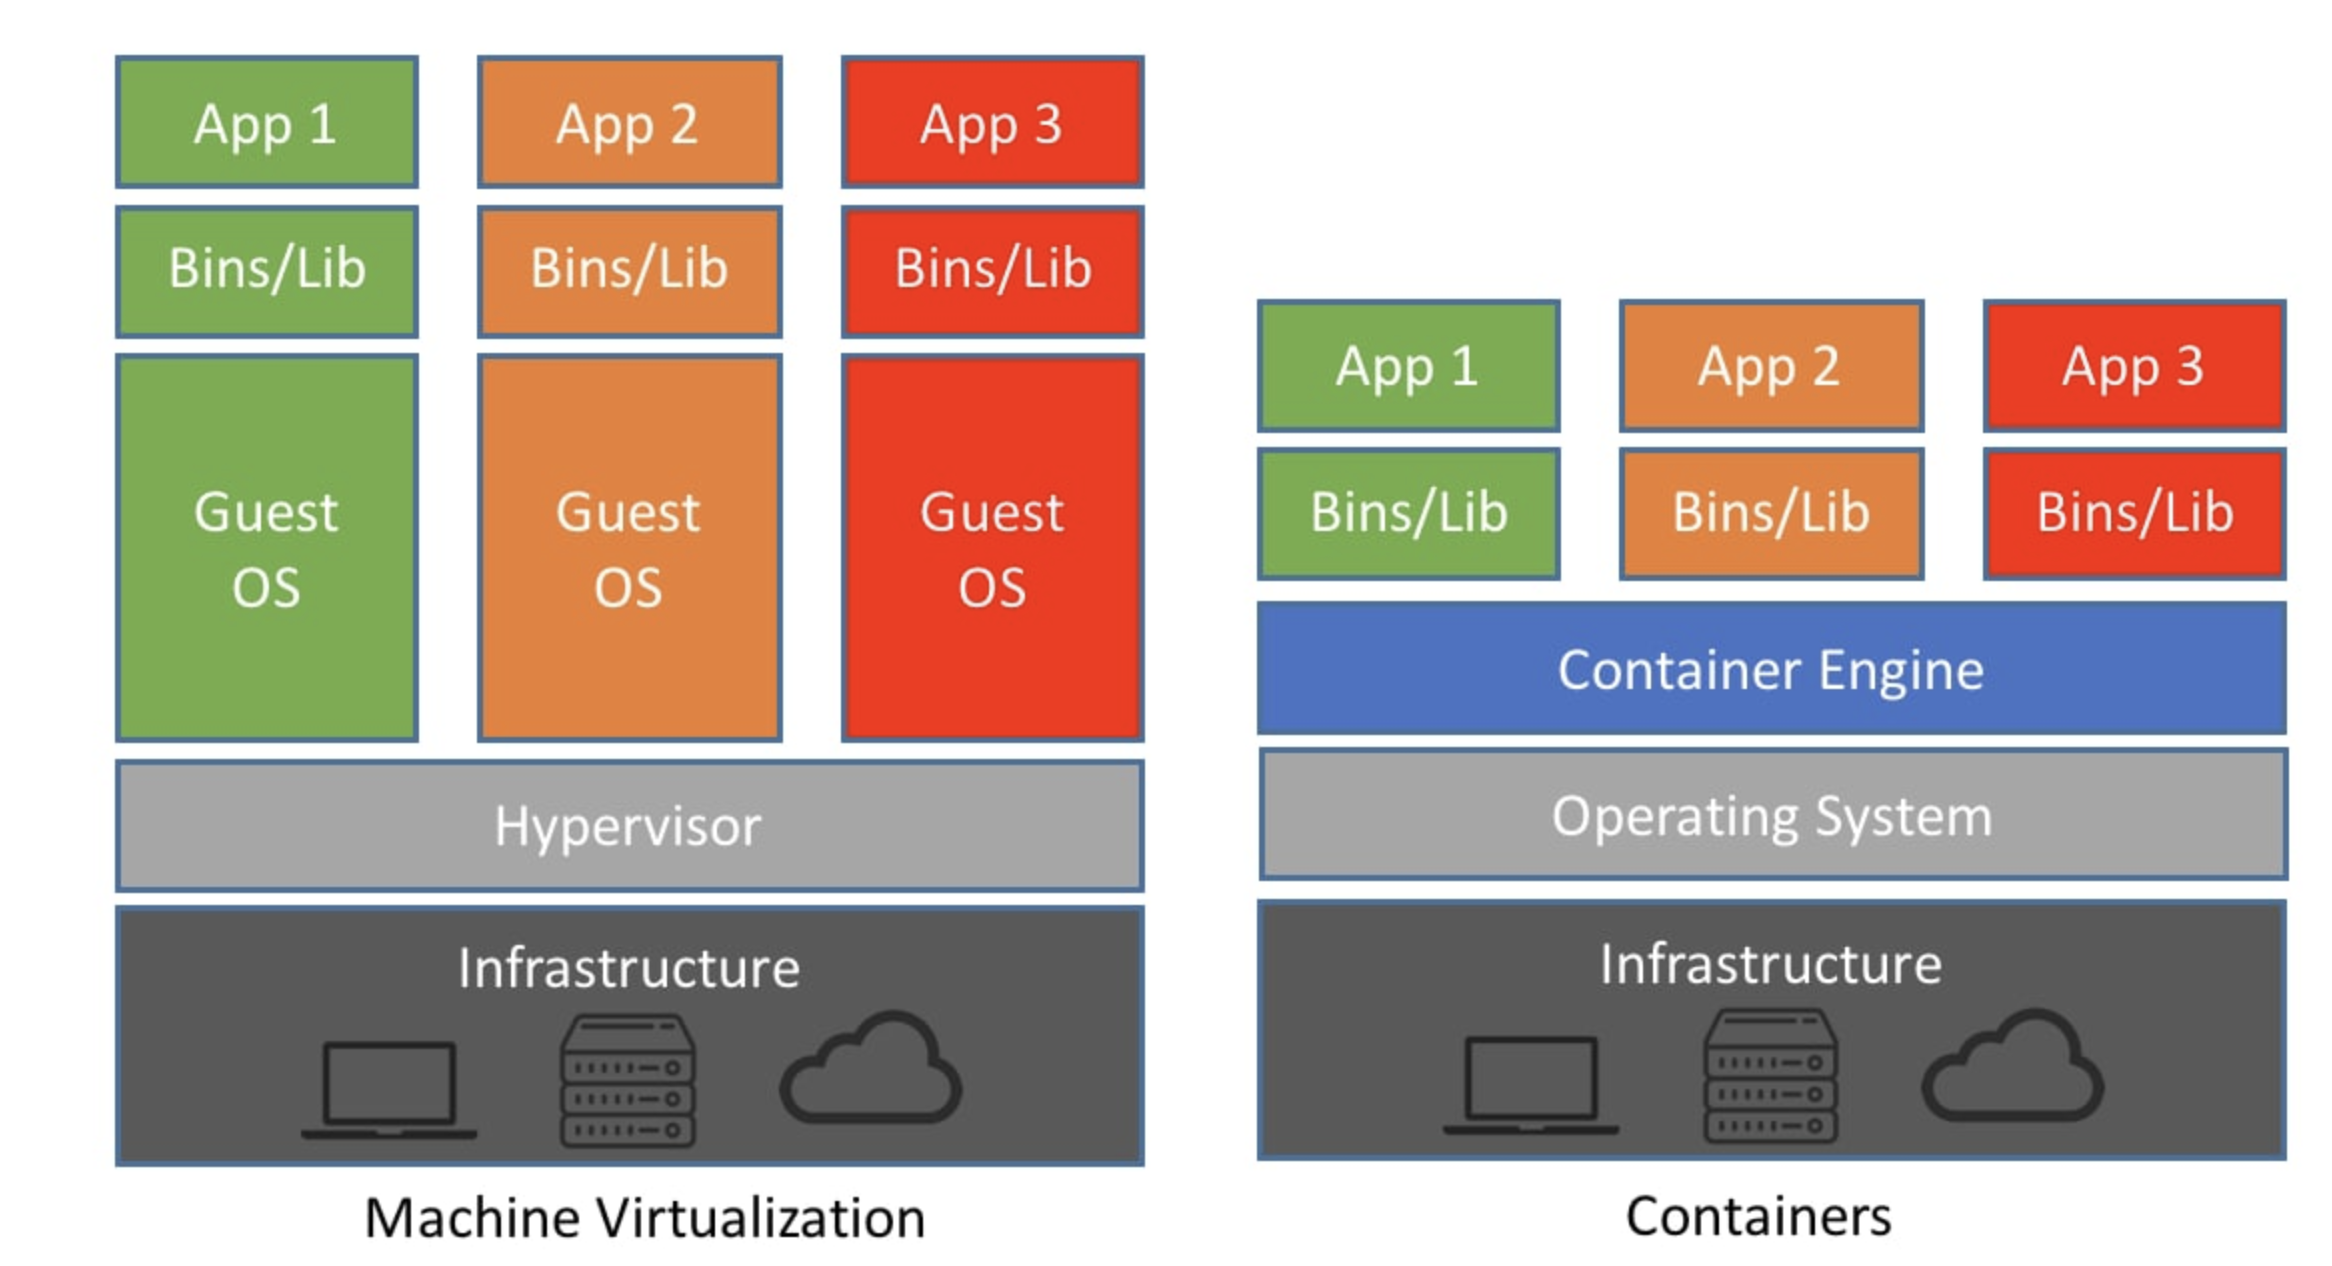
\includegraphics[width=0.9\textwidth, height=0.7\textheight, keepaspectratio]
            {figures/13_vm.png}
    \end{center}

    \vspace{0.1cm}
    \begin{center}
        \tiny\textcolor{gray}{Sumber: NetApp -- containers-vs-vms}
    \end{center}
\end{frame}

%--- Slide 3: Perbandingan ---
\begin{frame}[shrink=5]
    \frametitle{Perbandingan Langsung}

    \begin{center}
        \small
        \begin{tabular}{p{0.23\textwidth}p{0.33\textwidth}p{0.33\textwidth}}
            \toprule
            \textbf{Aspek} & \textbf{Virtual Machine} & \textbf{Container} \\
            \midrule
            Boot time & Menit & Detik \\
            Ukuran & GB (OS penuh) & MB (aplikasi + lib) \\
            Isolasi & Kuat (hardware level) & Level proses (namespace) \\
            Resource & Boros (setiap VM punya OS) & Hemat (pakai kernel host) \\
            Portability & Image besar, pindah lambat & Image kecil, mudah deploy \\
            Use case & Butuh OS berbeda, multi-tenant & Microservices, CI/CD, dev env \\
            \bottomrule
        \end{tabular}
    \end{center}

    \vspace{0.2cm}
    \begin{exampleblock}{Kapan Pilih Mana?}
        \small
        \begin{itemize}
            \item Butuh jalan aplikasi Linux di Windows server? $\to$ VM.
            \item Butuh deploy 20 microservices di satu server? $\to$ Container.
        \end{itemize}
    \end{exampleblock}
\end{frame}

%--- Slide 4: Docker Basics ---
\begin{frame}[fragile, shrink=10]
    \frametitle{Docker Basics: Image, Container, Dockerfile}
    \framesubtitle{Tiga konsep inti Docker}

    \begin{columns}[T]
        \column{0.48\textwidth}
        \begin{block}{Image}
            \small
            \begin{itemize}
                \item Template read-only yang berisi aplikasi + semua dependensinya.
                \item Bisa di-download dari registry (Docker Hub).
                \item Seperti ``CD installer'' -- tidak bisa diubah.
            \end{itemize}
        \end{block}

        \vspace{0.1cm}
        \begin{block}{Container}
            \small
            \begin{itemize}
                \item Instance jalan dari sebuah image.
                \item Bisa dibuat, distart, distop, dihapus.
                \item Seperti ``komputer virtual'' mini yang jalan di atas host.
            \end{itemize}
        \end{block}

        \column{0.48\textwidth}
        \begin{block}{Dockerfile}
            \small
            \begin{itemize}
                \item Resep untuk membangun image.
                \item Berisi perintah: ambil base image, copy file, install, dsb.
            \end{itemize}
        \end{block}

        \vspace{0.05cm}
        \begin{exampleblock}{Command Penting}
            \small
            \texttt{docker pull ubuntu} \\
            \texttt{docker run -it ubuntu bash} \\
            \texttt{docker build -t myapp .} \\
            \texttt{docker ps} \\
            \texttt{docker stop <id>}
        \end{exampleblock}
    \end{columns}
\end{frame}

%--- Slide 5: Contoh Dockerfile ---
\begin{frame}[fragile, shrink=5]
    \frametitle{Contoh Dockerfile Sederhana}
    \framesubtitle{Web server statis dengan Nginx}

    \tiny
    \begin{columns}[T]
        \column{0.55\textwidth}
        \begin{lstlisting}[basicstyle=\ttfamily\tiny, breaklines=true]
# Ambil base image resmi Nginx
FROM nginx:alpine

# Copy file HTML ke direktori default Nginx
COPY index.html /usr/share/nginx/html/

# Ekspos port 80
EXPOSE 80

# Perintah jalan saat container start
CMD ["nginx", "-g", "daemon off;"]
        \end{lstlisting}

        \column{0.40\textwidth}
        \begin{block}{Penjelasan}
            \tiny
            \begin{itemize}
                \item \texttt{FROM} -- base image yang sudah ada OS + Nginx.
                \item \texttt{COPY} -- masukkan file kita ke dalam image.
                \item \texttt{EXPOSE} -- kasih tahu container ini buka port 80.
                \item \texttt{CMD} -- perintah yang jalan saat container start.
            \end{itemize}
        \end{block}
    \end{columns}

    \vspace{0.15cm}
    \begin{exampleblock}{Build \& Run}
        \small
        \texttt{\$ docker build -t my-nginx .} \hfill build image \\
        \texttt{\$ docker run -d -p 8080:80 my-nginx} \hfill jalan container
    \end{exampleblock}
\end{frame}

%--- Slide 6: Isolasi Container ---
\begin{frame}[shrink=10]
    \frametitle{Bagaimana Container Isolasi?}
    \framesubtitle{Namespaces dan Cgroups -- ``Dua Pilar'' Docker}

    \begin{columns}[T]
        \column{0.48\textwidth}
        \begin{block}{Namespaces (Pemisahan)}
            \small
            Setiap container punya ``tampilan'' sendiri terhadap sistem:
            \begin{itemize}
                \item \texttt{PID ns} -- hanya lihat proses di dalam container.
                \item \texttt{NET ns} -- network interface sendiri, IP sendiri.
                \item \texttt{MNT ns} -- file system root sendiri.
                \item \texttt{UTS ns} -- hostname sendiri.
                \item \texttt{USER ns} -- user ID sendiri (bisa root di dalam).
            \end{itemize}
        \end{block}

        \column{0.48\textwidth}
        \begin{block}{Cgroups (Batas Sumber Daya)}
            \small
            \begin{itemize}
                \item Membatasi CPU, memory, disk I/O per container.
                \item Satu container tidak bisa ``makan'' semua resource.
                \item Contoh: \\
                \texttt{docker run --memory=256m --cpus=1.5 ...}
            \end{itemize}
        \end{block}
    \end{columns}

    \vspace{0.2cm}
    \begin{exampleblock}{Intuisi: Container = Proses + ``Kacamata Kuda''}
        \small
        Container adalah proses biasa, tapi OS memakai namespace untuk membuatnya ``lihat'' dunia yang terisolasi -- seolah-olah dia sendiri di komputer itu.
    \end{exampleblock}
\end{frame}

%--- Checkpoint 3 ---
\begin{frame}
    \frametitle{Checkpoint 3}
    \framesubtitle{Docker -- Cek pemahaman}
    \small
    \begin{enumerate}
        \item Apa perbedaan image dan container?
        \item Kenapa container lebih ringan dari VM?
        \item Dua mekanisme OS apa yang membuat container bisa isolasi?
    \end{enumerate}
    \vspace{0.3cm}
    \begin{block}{Jawaban Singkat}
        \begin{enumerate}
            \item Image = template read-only; Container = instance jalan dari image.
            \item Container pakai kernel host bersama, tidak perlu Guest OS sendiri.
            \item Namespaces (pemisahan tampilan) dan Cgroups (pembatasan resource).
        \end{enumerate}
    \end{block}
\end{frame}

%================================================
% BAGIAN 4: RAID
%================================================
\section{RAID \& Storage Redundancy}

%--- Slide 1: Motivasi ---
\begin{frame}
    \frametitle{Masalah: Satu Disk Rusak, Data Hilang}
    \framesubtitle{Kenapa kita butuh redundansi penyimpanan?}

    \begin{columns}[T]
        \column{0.48\textwidth}
        \begin{alertblock}{Masalah Nyata}
            \small
            \begin{itemize}
                \item Hard disk memiliki \textit{MTBF} (Mean Time Before Failure) -- rata-rata 3--5 tahun.
                \item Dalam data center dengan 1.000 disk, satu disk rusak hampir setiap minggu.
                \item Satu disk rusak $\to$ semua data di disk itu lenyap.
                \item Solusi naif: backup manual -- lambat dan tidak real-time.
            \end{itemize}
        \end{alertblock}

        \column{0.48\textwidth}
        \begin{exampleblock}{Analogi: Dua Motor}
            \small
            \begin{itemize}
                \item Bayangkan kita pergi naik motor. Ban motor bisa bocor kapan saja.
                \item Tanpa cadangan: kita berhenti total dan harus panggil tukang tambal.
                \item Dengan ban cadangan: kita ganti dan lanjut perjalanan.
                \item \textbf{RAID} adalah ``ban cadangan'' untuk hard disk -- jika satu rusak, yang lain langsung menggantikan.
            \end{itemize}
        \end{exampleblock}
    \end{columns}
\end{frame}

%--- Slide 2a: RAID 0 -- Cara Kerja ---
\begin{frame}[shrink=5]
    \frametitle{RAID 0: Striping (1/2)}
    \framesubtitle{Data dipecah dan disebar ke beberapa disk}

    \begin{columns}[T]
        \column{0.40\textwidth}
        \begin{block}{Cara Kerja}
            \small
            \begin{itemize}
                \item Data dipecah (\textit{striped}) menjadi potongan-potongan kecil.
                \item Potongan disebar ke beberapa disk secara bergantian.
                \item Membaca/menulis bisa paralel $\to$ lebih cepat.
                \item Dibutuhkan minimal 2 disk.
            \end{itemize}
        \end{block}

        \column{0.56\textwidth}
        \begin{center}
            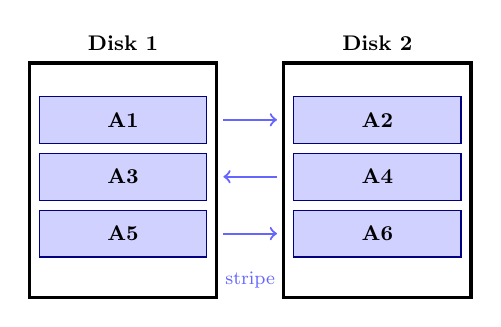
\begin{tikzpicture}[scale=0.85, transform shape]
                % Disk 1
                \draw[very thick] (0,0) rectangle (2.8, -3.5);
                \node[font=\bfseries\small] at (1.4, 0.3) {Disk 1};
                \draw[fill=blue!18, draw=blue!50!black] (0.15,-0.5) rectangle (2.65, -1.2);
                \node[font=\small\bfseries] at (1.4, -0.85) {A1};
                \draw[fill=blue!18, draw=blue!50!black] (0.15,-1.35) rectangle (2.65, -2.05);
                \node[font=\small\bfseries] at (1.4, -1.7) {A3};
                \draw[fill=blue!18, draw=blue!50!black] (0.15,-2.2) rectangle (2.65, -2.9);
                \node[font=\small\bfseries] at (1.4, -2.55) {A5};
                % Disk 2
                \draw[very thick] (3.8,0) rectangle (6.6, -3.5);
                \node[font=\bfseries\small] at (5.2, 0.3) {Disk 2};
                \draw[fill=blue!18, draw=blue!50!black] (3.95,-0.5) rectangle (6.45, -1.2);
                \node[font=\small\bfseries] at (5.2, -0.85) {A2};
                \draw[fill=blue!18, draw=blue!50!black] (3.95,-1.35) rectangle (6.45, -2.05);
                \node[font=\small\bfseries] at (5.2, -1.7) {A4};
                \draw[fill=blue!18, draw=blue!50!black] (3.95,-2.2) rectangle (6.45, -2.9);
                \node[font=\small\bfseries] at (5.2, -2.55) {A6};
                % Arrows
                \draw[->, thick, blue!60] (2.9, -0.85) -- (3.7, -0.85);
                \draw[->, thick, blue!60] (3.7, -1.7) -- (2.9, -1.7);
                \draw[->, thick, blue!60] (2.9, -2.55) -- (3.7, -2.55);
                \node[font=\footnotesize, blue!60] at (3.3, -3.25) {stripe};
            \end{tikzpicture}
        \end{center}
    \end{columns}
\end{frame}

%--- Slide 2b: RAID 0 -- Risiko ---
\begin{frame}[shrink=5]
    \frametitle{RAID 0: Striping (2/2)}
    \framesubtitle{Risiko dan kapan sebaiknya digunakan}

    \begin{columns}[T]
        \column{0.48\textwidth}
        \begin{alertblock}{Risiko}
            \small
            \begin{itemize}
                \item \textbf{Tidak ada redundansi!}
                \item Jika satu disk rusak $\to$ \tem{semua data hilang}.
                \item Probabilitas failure = $N \times P$ (lebih besar dari disk tunggal).
            \end{itemize}
        \end{alertblock}

        \column{0.48\textwidth}
        \begin{block}{Kapan Dipakai?}
            \small
            \begin{itemize}
                \item Video editing (butuh throughput tinggi).
                \item Data sementara yang bisa di-recreate.
            \end{itemize}
        \end{block}
    \end{columns}
\end{frame}

%--- Slide 3a: RAID 1 -- Cara Kerja ---
\begin{frame}[shrink=5]
    \frametitle{RAID 1: Mirroring (1/2)}
    \framesubtitle{Data ditulis identik ke dua disk}

    \begin{columns}[T]
        \column{0.40\textwidth}
        \begin{block}{Cara Kerja}
            \small
            \begin{itemize}
                \item Setiap data ditulis ke \textbf{dua disk} secara identik (\textit{mirror}).
                \item Jika Disk 1 rusak, Disk 2 masih punya salinan lengkap.
                \item Baca bisa paralel (lebih cepat), tulis tetap ke dua disk.
                \item Dibutuhkan minimal 2 disk.
            \end{itemize}
        \end{block}

        \column{0.56\textwidth}
        \begin{center}
            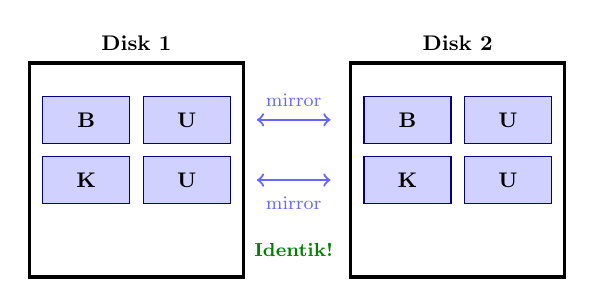
\begin{tikzpicture}[scale=0.85, transform shape]
                % Disk 1
                \draw[very thick] (0,0) rectangle (3.2, -3.2);
                \node[font=\bfseries\small] at (1.6, 0.3) {Disk 1};
                \draw[fill=blue!18, draw=blue!50!black] (0.2,-0.5) rectangle (1.5, -1.2);
                \node[font=\small\bfseries] at (0.85, -0.85) {B};
                \draw[fill=blue!18, draw=blue!50!black] (1.7,-0.5) rectangle (3.0, -1.2);
                \node[font=\small\bfseries] at (2.35, -0.85) {U};
                \draw[fill=blue!18, draw=blue!50!black] (0.2,-1.4) rectangle (1.5, -2.1);
                \node[font=\small\bfseries] at (0.85, -1.75) {K};
                \draw[fill=blue!18, draw=blue!50!black] (1.7,-1.4) rectangle (3.0, -2.1);
                \node[font=\small\bfseries] at (2.35, -1.75) {U};

                % Arrows mirror
                \draw[<->, thick, blue!60] (3.4, -0.85) -- (4.5, -0.85);
                \draw[<->, thick, blue!60] (4.5, -1.75) -- (3.4, -1.75);
                \node[font=\footnotesize, blue!60] at (3.95, -0.55) {mirror};
                \node[font=\footnotesize, blue!60] at (3.95, -2.1) {mirror};

                % Disk 2
                \draw[very thick] (4.8,0) rectangle (8.0, -3.2);
                \node[font=\bfseries\small] at (6.4, 0.3) {Disk 2};
                \draw[fill=blue!18, draw=blue!50!black] (5.0,-0.5) rectangle (6.3, -1.2);
                \node[font=\small\bfseries] at (5.65, -0.85) {B};
                \draw[fill=blue!18, draw=blue!50!black] (6.5,-0.5) rectangle (7.8, -1.2);
                \node[font=\small\bfseries] at (7.15, -0.85) {U};
                \draw[fill=blue!18, draw=blue!50!black] (5.0,-1.4) rectangle (6.3, -2.1);
                \node[font=\small\bfseries] at (5.65, -1.75) {K};
                \draw[fill=blue!18, draw=blue!50!black] (6.5,-1.4) rectangle (7.8, -2.1);
                \node[font=\small\bfseries] at (7.15, -1.75) {U};

                % Label identik
                \node[font=\footnotesize, green!50!black, align=center] at (3.95, -2.8) {{\bf Identik!}};
            \end{tikzpicture}
        \end{center}
    \end{columns}
\end{frame}

%--- Slide 3b: RAID 1 -- Kekurangan ---
\begin{frame}[shrink=5]
    \frametitle{RAID 1: Mirroring (2/2)}
    \framesubtitle{Kekurangan dan kapan sebaiknya digunakan}

    \begin{columns}[T]
        \column{0.48\textwidth}
        \begin{alertblock}{Kekurangan}
            \small
            \begin{itemize}
                \item \textbf{Kapasitas terpakai hanya 50\%}.
                \item 2 TB (2 disk $\times$ 1 TB) = hanya 1 TB yang terpakai.
            \end{itemize}
        \end{alertblock}

        \column{0.48\textwidth}
        \begin{block}{Kapan Dipakai?}
            \small
            \begin{itemize}
                \item Sistem kritis (OS, database log).
                \item Data yang tidak boleh hilang.
            \end{itemize}
        \end{block}
    \end{columns}
\end{frame}

%--- Slide 4a: RAID 5 -- Cara Kerja ---
\begin{frame}[shrink=5]
    \frametitle{RAID 5: Parity (1/3)}
    \framesubtitle{Data + parity disebar ke semua disk}

    \begin{columns}[T]
        \column{0.40\textwidth}
        \begin{block}{Cara Kerja RAID 5}
            \small
            \begin{itemize}
                \item Data + \textit{parity} (informasi pemulihan) disebar ke semua disk.
                \item Parity memakan kapasitas \textbf{1 disk}.
                \item 3 disk (3 TB) $\to$ 2 TB data + 1 TB parity.
                \item Tahan terhadap \textbf{1 disk} rusak.
                \item Write lebih lambat karena harus hitung parity.
            \end{itemize}
        \end{block}

        \column{0.56\textwidth}
        \begin{center}
            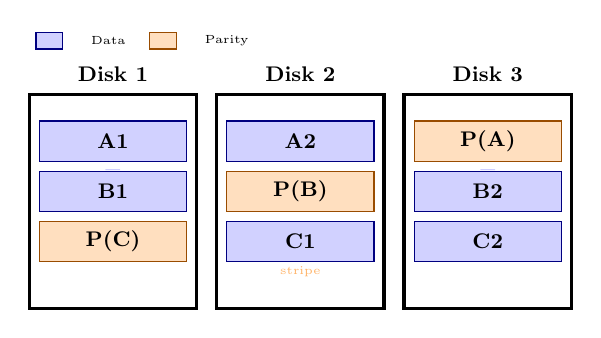
\begin{tikzpicture}[scale=0.85, transform shape]
                % Legend
                \node[fill=blue!18, draw=blue!50!black, minimum width=0.4cm, minimum height=0.25cm] at (0.3, 0.8) {};
                \node[font=\tiny, anchor=west] at (0.8, 0.8) {Data};
                \node[fill=orange!25, draw=orange!60!black, minimum width=0.4cm, minimum height=0.25cm] at (2.0, 0.8) {};
                \node[font=\tiny, anchor=west] at (2.5, 0.8) {Parity};

                % Disk 1
                \draw[very thick] (0,0) rectangle (2.5, -3.2);
                \node[font=\bfseries\small] at (1.25, 0.3) {Disk 1};
                \draw[fill=blue!18, draw=blue!50!black] (0.15,-0.4) rectangle (2.35, -1.0);
                \node[font=\small\bfseries] at (1.25, -0.7) {A1};
                \draw[fill=blue!18, draw=blue!50!black] (0.15,-1.15) rectangle (2.35, -1.75);
                \node[font=\small\bfseries] at (1.25, -1.45) {B1};
                \draw[fill=orange!25, draw=orange!60!black] (0.15,-1.9) rectangle (2.35, -2.5);
                \node[font=\small\bfseries] at (1.25, -2.2) {P(C)};

                % Disk 2
                \draw[very thick] (2.8,0) rectangle (5.3, -3.2);
                \node[font=\bfseries\small] at (4.05, 0.3) {Disk 2};
                \draw[fill=blue!18, draw=blue!50!black] (2.95,-0.4) rectangle (5.15, -1.0);
                \node[font=\small\bfseries] at (4.05, -0.7) {A2};
                \draw[fill=orange!25, draw=orange!60!black] (2.95,-1.15) rectangle (5.15, -1.75);
                \node[font=\small\bfseries] at (4.05, -1.45) {P(B)};
                \draw[fill=blue!18, draw=blue!50!black] (2.95,-1.9) rectangle (5.15, -2.5);
                \node[font=\small\bfseries] at (4.05, -2.2) {C1};

                % Disk 3
                \draw[very thick] (5.6,0) rectangle (8.1, -3.2);
                \node[font=\bfseries\small] at (6.85, 0.3) {Disk 3};
                \draw[fill=orange!25, draw=orange!60!black] (5.75,-0.4) rectangle (7.95, -1.0);
                \node[font=\small\bfseries] at (6.85, -0.7) {P(A)};
                \draw[fill=blue!18, draw=blue!50!black] (5.75,-1.15) rectangle (7.95, -1.75);
                \node[font=\small\bfseries] at (6.85, -1.45) {B2};
                \draw[fill=blue!18, draw=blue!50!black] (5.75,-1.9) rectangle (7.95, -2.5);
                \node[font=\small\bfseries] at (6.85, -2.2) {C2};

                % Parity label per stripe
                \node[font=\tiny, blue!60] at (1.25, -1.15) {---};
                \node[font=\tiny, blue!60] at (6.85, -1.15) {---};
                \node[font=\tiny, orange!60] at (4.05, -2.65) {stripe};
            \end{tikzpicture}
        \end{center}
    \end{columns}
\end{frame}

%--- Slide 4b: RAID 6 -- Cara Kerja ---
\begin{frame}[shrink=5]
    \frametitle{RAID 6: Parity Ganda (2/3)}
    \framesubtitle{Dua parity (P + Q) untuk redundansi ganda}

    \begin{columns}[T]
        \column{0.40\textwidth}
        \begin{block}{Cara Kerja RAID 6}
            \small
            \begin{itemize}
                \item Dua parity (P + Q) -- redundansi ganda.
                \item Parity memakan kapasitas \textbf{2 disk}.
                \item Tahan terhadap \textbf{2 disk} rusak \textbf{bersamaan}.
                \item Cocok untuk disk besar dengan rebuild time lama.
            \end{itemize}
        \end{block}

        \column{0.56\textwidth}
        \begin{center}
            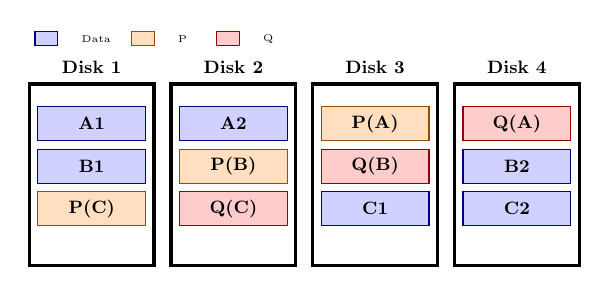
\begin{tikzpicture}[scale=0.72, transform shape]
                % Legend
                \node[fill=blue!18, draw=blue!50!black, minimum width=0.4cm, minimum height=0.25cm] at (0.3, 0.8) {};
                \node[font=\tiny, anchor=west] at (0.8, 0.8) {Data};
                \node[fill=orange!25, draw=orange!60!black, minimum width=0.4cm, minimum height=0.25cm] at (2.0, 0.8) {};
                \node[font=\tiny, anchor=west] at (2.5, 0.8) {P};
                \node[fill=red!20, draw=red!60!black, minimum width=0.4cm, minimum height=0.25cm] at (3.5, 0.8) {};
                \node[font=\tiny, anchor=west] at (4.0, 0.8) {Q};

                % Disk 1
                \draw[very thick] (0,0) rectangle (2.2, -3.2);
                \node[font=\bfseries\small] at (1.1, 0.3) {Disk 1};
                \draw[fill=blue!18, draw=blue!50!black] (0.15,-0.4) rectangle (2.05, -1.0);
                \node[font=\small\bfseries] at (1.1, -0.7) {A1};
                \draw[fill=blue!18, draw=blue!50!black] (0.15,-1.15) rectangle (2.05, -1.75);
                \node[font=\small\bfseries] at (1.1, -1.45) {B1};
                \draw[fill=orange!25, draw=orange!60!black] (0.15,-1.9) rectangle (2.05, -2.5);
                \node[font=\small\bfseries] at (1.1, -2.2) {P(C)};

                % Disk 2
                \draw[very thick] (2.5,0) rectangle (4.7, -3.2);
                \node[font=\bfseries\small] at (3.6, 0.3) {Disk 2};
                \draw[fill=blue!18, draw=blue!50!black] (2.65,-0.4) rectangle (4.55, -1.0);
                \node[font=\small\bfseries] at (3.6, -0.7) {A2};
                \draw[fill=orange!25, draw=orange!60!black] (2.65,-1.15) rectangle (4.55, -1.75);
                \node[font=\small\bfseries] at (3.6, -1.45) {P(B)};
                \draw[fill=red!20, draw=red!60!black] (2.65,-1.9) rectangle (4.55, -2.5);
                \node[font=\small\bfseries] at (3.6, -2.2) {Q(C)};

                % Disk 3
                \draw[very thick] (5.0,0) rectangle (7.2, -3.2);
                \node[font=\bfseries\small] at (6.1, 0.3) {Disk 3};
                \draw[fill=orange!25, draw=orange!60!black] (5.15,-0.4) rectangle (7.05, -1.0);
                \node[font=\small\bfseries] at (6.1, -0.7) {P(A)};
                \draw[fill=red!20, draw=red!60!black] (5.15,-1.15) rectangle (7.05, -1.75);
                \node[font=\small\bfseries] at (6.1, -1.45) {Q(B)};
                \draw[fill=blue!18, draw=blue!50!black] (5.15,-1.9) rectangle (7.05, -2.5);
                \node[font=\small\bfseries] at (6.1, -2.2) {C1};

                % Disk 4
                \draw[very thick] (7.5,0) rectangle (9.7, -3.2);
                \node[font=\bfseries\small] at (8.6, 0.3) {Disk 4};
                \draw[fill=red!20, draw=red!60!black] (7.65,-0.4) rectangle (9.55, -1.0);
                \node[font=\small\bfseries] at (8.6, -0.7) {Q(A)};
                \draw[fill=blue!18, draw=blue!50!black] (7.65,-1.15) rectangle (9.55, -1.75);
                \node[font=\small\bfseries] at (8.6, -1.45) {B2};
                \draw[fill=blue!18, draw=blue!50!black] (7.65,-1.9) rectangle (9.55, -2.5);
                \node[font=\small\bfseries] at (8.6, -2.2) {C2};
            \end{tikzpicture}
        \end{center}
    \end{columns}
\end{frame}

%--- Slide 4c: RAID 5 & 6 -- Analogi ---
\begin{frame}[shrink=5]
    \frametitle{RAID 5 \& 6: Analogi Parity (3/3)}
    \framesubtitle{Bagaimana parity bekerja?}

    \begin{columns}[T]
        \column{0.48\textwidth}
        \begin{exampleblock}{Analogi: Permainan Teka-Teki}
            \small
            \begin{itemize}
                \item Parity seperti \textbf{petunjuk} dalam teka-teki silang.
                \item Jika satu kotak hilang, kita masih bisa menebak isinya dari petunjuk baris dan kolom yang lain.
                \item \textbf{RAID 5} = satu petunjuk -- satu kotak hilang masih tertebak.
                \item \textbf{RAID 6} = dua petunjuk -- dua kotak hilang pun masih tertebak.
            \end{itemize}
        \end{exampleblock}

        \column{0.48\textwidth}
        \begin{block}{Mengapa Parity Penting?}
            \small
            \begin{itemize}
                \item RAID 5 hanya butuh \textbf{1 disk ekstra} untuk mengamankan \textbf{banyak disk}.
                \item RAID 6 butuh \textbf{2 disk ekstra} tapi tahan 2 kerusakan.
                \item Lebih efisien dari RAID 1 (50\%) untuk data besar.
                \item Kekurangan: write lebih lambat karena harus hitung parity.
            \end{itemize}
        \end{block}
    \end{columns}
\end{frame}

%--- Slide 5: Perbandingan ---
\begin{frame}[shrink=5]
    \frametitle{Perbandingan RAID Levels}

    \begin{center}
        \resizebox{\textwidth}{!}{
        \begin{tabular}{p{0.18\textwidth}p{0.17\textwidth}p{0.17\textwidth}p{0.17\textwidth}p{0.17\textwidth}}
            \toprule
            \textbf{Aspek} & \textbf{RAID 0} & \textbf{RAID 1} & \textbf{RAID 5} & \textbf{RAID 6} \\
            \midrule
            Minimal disk & 2 & 2 & 3 & 4 \\
            Redundansi & Tidak ada & Salinan penuh & Parity (1) & Parity ganda (2) \\
            Tahan rusak & 0 disk & 1 disk & 1 disk & 2 disk \\
            Kapasitas & 100\% & 50\% & $(N-1)/N$ & $(N-2)/N$ \\
            Baca & Sangat cepat & Cepat & Cepat & Cepat \\
            Tulis & Sangat cepat & Sedang & Lambat & Paling lambat \\
            Biaya & Murah & Mahal & Sedang & Sedang \\
            \bottomrule
        \end{tabular}
        }
    \end{center}

    \vspace{0.2cm}
    \begin{block}{Tips Memilih}
        \small
        \begin{itemize}
            \item Prioritaskan kecepatan? $\to$ RAID 0 (tapi backup terpisah wajib!)
            \item Prioritaskan keamanan? $\to$ RAID 1 (data kecil) atau RAID 5/6 (data besar)
        \end{itemize}
    \end{block}
\end{frame}

%--- Checkpoint 4 ---
\begin{frame}
    \frametitle{Checkpoint 4}
    \framesubtitle{RAID -- Cek pemahaman}
    \small
    \begin{enumerate}
        \item Bedanya RAID 0 dan RAID 1?
        \item Kenapa RAID 5 lebih efisien kapasitasnya daripada RAID 1?
        \item Kapan kita butuh RAID 6 daripada RAID 5?
    \end{enumerate}
    \vspace{0.3cm}
    \begin{block}{Jawaban Singkat}
        \begin{enumerate}
            \item RAID 0 = striping (cepat, tanpa redundansi); RAID 1 = mirroring (aman, kapasitas setengah).
            \item RAID 5 hanya kehilangan kapasitas 1 disk untuk parity, bukan setengah dari total.
            \item Saat pakai disk besar (recovery lama) -- dua disk bisa rusak dalam waktu pemulihan.
        \end{enumerate}
    \end{block}
\end{frame}

%================================================
% PENUTUP
%================================================
\section*{Penutup}

\begin{frame}[shrink=5]
    \frametitle{Rangkuman Hari Ini}
    \small
    \begin{enumerate}
        \item \textbf{Hak Akses}: Unix membagi izin r/w/x untuk Owner, Group, Others. Ditambah special bits SUID/SGID/Sticky.
        \item \textbf{Keamanan OS}: Malware (virus, worm, trojan, ransomware) dan mekanisme proteksi OS (user/kernel mode, ASLR, NX bit, isolasi address space).
        \item \textbf{Docker}: Container sebagai OS-level virtualization yang ringan. Namespace dan Cgroups sebagai kunci isolasi.
        \item \textbf{RAID}: Redundansi penyimpanan lewat striping (RAID 0), mirroring (RAID 1), atau parity (RAID 5/6).
    \end{enumerate}

    \vspace{0.2cm}
    \begin{exampleblock}{Pesan Penutup}
        \small
        Materi pekan depan: \textbf{Quiz}! Persiapkan diri dari Week 1--13.
    \end{exampleblock}
\end{frame}

%--- Penutup ---
\begin{frame}
    \frametitle{Terima Kasih}
    \begin{center}
        \Huge \textbf{Ada Pertanyaan?}

        \vspace{0.8cm}
        \normalsize
        Selamat belajar dan tetap aman di dunia maya!

        \vspace{0.8cm}
        \small
        \textit{``The only secure system is the one that is powered off, sheathed in a block of concrete and sealed in a lead-lined room with armed guards.''} \\
        \vspace{0.1cm}
        --- Gene Spafford
    \end{center}
\end{frame}

\end{document}
